\documentclass[12pt]{article}
\usepackage{amsmath}
\usepackage{amsthm}
\usepackage{graphicx,psfrag,epsf}
\usepackage{enumerate}
\usepackage{natbib}
\usepackage{url} % not crucial - just used below for the URL
\usepackage{color}


%\pdfminorversion=4
% NOTE: To produce blinded version, replace "0" with "1" below.
\newcommand{\blind}{0}

% DON'T change margins - should be 1 inch all around.
\addtolength{\oddsidemargin}{-.5in}%
\addtolength{\evensidemargin}{-.5in}%
\addtolength{\textwidth}{1in}%
\addtolength{\textheight}{1.3in}%
\addtolength{\topmargin}{-.8in}%


%%%% Packages and definitions
\usepackage{amssymb}

\usepackage{xr}

\usepackage[top=0.85in,left=1.0in,right=1.0in,footskip=0.75in]{geometry}

% Use adjustwidth environment to exceed column width (see example table in text)
\usepackage{changepage}

% Use Unicode characters when possible
\usepackage[utf8]{inputenc}

% textcomp package and marvosym package for additional characters
\usepackage{textcomp,marvosym}

\usepackage[ruled]{algorithm}
\usepackage{algorithmic}

% cite package, to clean up citations in the main text. Do not remove.
\usepackage{cite}

% Use nameref to cite supporting information files (see Supporting Information section for more info)
\usepackage{nameref,hyperref}

%\usepackage{amsthm}

% ligatures disabled
\usepackage{microtype}
\DisableLigatures[f]{encoding = *, family = * }

% for the beautiful checkmarks
\usepackage{pifont}

\newtheorem{theorem}{Theorem}
\newtheorem{corollary}{Corollary}
\newtheorem{lemma}{Lemma}
\newtheorem{definition}{Definition}
\newtheorem{condition}{Condition}

\DeclareMathOperator*{\argmin}{arg\,min}


\begin{document}

\def\spacingset#1{\renewcommand{\baselinestretch}%
{#1}\small\normalsize} \spacingset{1}


%%%%%%%%%%%%%%%%%%%%%%%%%%%%%%%%%%%%%%%%%%%%%%%%%%%%%%%%%%%%%%%%%%%%%%%%%%%%%%

\if0\blind
{
  \title{\bf Oracle Inequalities for multiple penalty parameters}
  \author{Jean Feng\thanks{
    Jean Feng was supported by NIH grants ???. % DP5OD019820 and T32CA206089.
    Noah Simon was supported by NIH grant DP5OD019820.
    The content is solely the responsibility of the authors and does not necessarily represent the official views of the National Institutes of Health.}\\
    Department of Biostatistics, University of Washington\\
    and \\
    Noah Simon \\
    Department of Biostatistics, University of Washington}
  \maketitle
} \fi

\if1\blind
{
  \bigskip
  \bigskip
  \bigskip
  \begin{center}
    {\LARGE\bf Cross-validation for many penalty parameters.}
\end{center}
  \medskip
} \fi

\bigskip
\begin{abstract}

In penalized regression problems, the choice of penalty parameters is important since they ultimately determine the fitted model. The penalty parameters that minimize the generalization error are generally unknown and must be estimated. In this paper, we establish finite-sample oracle inequalities for models selected by a validation set approach. Our upper bounds on the model error depend on the oracle error and a near-parametric term. Therefore in settings where the oracle error shrinks at a sub-parametric rate, the number of penalty parameters can grow with the sample size without affecting the asymptotic convergence rate. Our oracle inequalities hold for penalized regression problems where the fitted models are smoothly parameterized by the penalty parameters. We show that this smoothness condition is satisfied by adding a ridge penalty to the training criterion.

\end{abstract}

\noindent%
{\it Keywords:}  Regression, Cross-validation, Regularization
\vfill

\newpage
\spacingset{1.45}
\section{Introduction}

Per the usual regression framework, we observe response $y \in \mathbb{R}$ and predictors $\boldsymbol {x} \in \mathbb{R}^p$. Suppose $y$ is generated from the model $g^*$ from model class $\mathcal{G}$
\begin{equation}
y = g^*(\boldsymbol x) + \epsilon
\end{equation}
where $\epsilon_i$ are random errors with expectation zero. Our goal is to find the best model in $\mathcal{G}$ to model $y$ given $\boldsymbol x$.

In high-dimensional ($p \gg n$) or ill-posed problems, the ordinary least squares estimate performs poorly as it overfits to the training data. A common solution is to add regularization, or penalization, to control model complexity and induce desired structure. The penalized least squares estimate minimizes a criterion of the form
\begin{equation}
\label{intro_train_criterion}
\hat{g}(\cdot | \boldsymbol \lambda) = \argmin_{g\in \mathcal{G}} \frac{1}{n} \sum_{i=1}^n \left (y_i -  g(x_i) \right )^2 + \sum_{j=1}^J \lambda_j P_j(g)
\end{equation}
where $P_j$ are the penalty functions and $\lambda_j$ are the penalty parameters.

Selecting the penalty parameters is an important task since they ultimately determine the fitted model. Their oracle values balance the residual least squares and the penalty terms to ensure fast convergence rates \citep{van2000empirical}. For example, when fitting an additive model $f(\boldsymbol x) = \sum_{j=1}^J f_j(x_j)$ with a roughness penalty for each component, the penalty parameters should be inversely proportional to the penalties of the true model \citep{van2014additive}. When fitting a linear model using the lasso, the penalty parameter should be on the order $\sigma (\log p /n )^{1/2}$ where $\sigma^2$ is the variance of the error terms \citep{buhlmann2011statistics}.

The obvious problem is that the oracle penalty parameters depend on unknown values. Thus penalty parameters are usually tuned via a training/validation split or cross-validation. The basic idea is to train a model on a random partition of the data and evaluate its error on the remaining data. The penalty parameters that minimize the error on this validation set are then selected. For a more complete review of cross-validation, refer to Arlot \citep{arlot2010survey}.

The performance of cross-validation-like procedures is typically characterized by an oracle inequality that bounds the error of the selected model. In a general cross-validation framework, \citet{van2003unified, van2004asymptotic} provides finite sample oracle inequalities assuming that cross-validation is performed over a finite model class and \citet{lecue2012oracle} uses an entropy approach to bound the error for cross-validated models from potentially infinite model classes. In the regression setting, \citet{gyorfi2006distribution} provides a finite sample inequality for training/validation split for least squares and \citet{wegkamp2003model} proves an oracle inequality for a penalized least squares holdout procedure. There are also bounds for cross-validated models from ridge regression and lasso \citep{golub1979generalized, chetverikov2016cross, chatterjee2015prediction}, though the proofs usually rely on the linearity of the model class and are therefore hard to generalize.

Despite the wealth of literature on cross-validation, there is very little work on characterizing the prediction error when the regularization method has multiple penalty parameters. A potential reason is that tuning multiple penalty parameters is computationally difficult; most regularization methods only have one or two tuning parameters (e.g. the Elastic Net and Sparse Group Lasso \citep{zou2003regression, simon2013sparse}). This computational hurdle has been addressed recently by using continuous optimization methods. For many penalized regression problems, the gradient of the validation loss with respect to the penalty parameters can be calculated using an implicit differentiation trick \citep{bengio2000gradient, foo2008efficient}. Thus a gradient descent procedure can be used to tune the penalty parameters. For more general ``hyperparameter selection'' problems, one can use a gradient-free approach such as Bayesian optimization \citet{snoek2012practical} or Nelder-Mead (CITE).

This paper provides a finite-sample upper bound on the prediction error when multiple penalty parameters are tuned via a training/validation split or cross-validation. We establish an upper bound on the model error that depends on the oracle error and a near-parametric term. Roughly speaking, the additional price for not knowing the oracle penalty parameters is a parametric term. For semi- and non-parametric regression problems, this term is generally much smaller than the oracle error and do not affect the asymptotic convergence rate. In fact, in these cases, the number of penalty parameters can grow with the sample size. Our oracle inequalities depend on the assumption that the fitted models are smoothly parameterized by the penalty parameters. We will show that this smoothness assumption can be easily satisfied if we add a ridge penalty to the training criterion. 
%The proofs rely on empirical process theory and the implicit differentiation trick in \citet{bengio2000gradient} and \citet{foo2008efficient}.

Section \ref{sec:main_results} provides bounds on the prediction error for a training/validation framework and cross-validation.
Section \ref{sec:examples} gives examples of penalized regression problems where the fitted models are smoothly parameterized by the penalty parameters.
Section \ref{sec:simulations} provides a simulation study to support our theoretical results.
Section \ref{sec:discussion} discusses our findings and potential future work.
Section \ref{sec:proofs} contains the proofs and other technical details.

\section{Main Result} \label{sec:main_results}

Suppose we have observations $D = \left \{ (\boldsymbol{x}_i, y_i) \right \}_{i=1}^n$ generated from the model
\begin{equation}
y_i = g^*(\boldsymbol x_i) + \epsilon_i \quad i=1,...,n
\end{equation}
where $g^*$ is from our model class $\mathcal{G}$ and $\epsilon_i$ are random variables with expectation zero. In the simple setting, one may assume that $\epsilon_i$ are normally distributed. Here we consider a more general situation where $\epsilon_1,...,\epsilon_n$ are uniformly sub-Gaussian random variables. We use the definition from \citep{Buldygin1980}:
\begin{definition}
	$\epsilon_1, ..., \epsilon_n$ are uniformly sub-Gaussian with parameter $b>0$ if for all $t \in \mathbb{R}$
	\begin{equation}
	\max_{i=1,...,n} \mathbb{E} e^{t \epsilon_i} \le e^{b^2t^2/2}
	\end{equation}
\end{definition}
Note that it is possible to show that if $\epsilon_1,...,\epsilon_n$ are uniformly sub-Gaussian, then they must have expectation zero \citep{stromberg1994probability}.

\subsection{Training/Validation Split}

Suppose dataset $D$ is randomly split into a training set $T$ of size $n_T$ and validation set $V$ of size $n_V$. For a function $h$, define $\| h \|_V^2 = \frac{1}{n_V}\sum_{i\in V} h^2(x_i)$ and similarly for $T$. Using this notation, the fitted model defined in  \eqref{intro_train_criterion} can be written as
\begin{equation}
\hat{g}(\cdot | \boldsymbol \lambda) = \argmin_{g\in \mathcal{G}} \frac{1}{2} \left \|y -  g \right \|_T^2 + \sum_{j=1}^J \lambda_j P_j(g)
\end{equation}

In the training/validation framework, we minimize the validation error by tuning over the range of possible penalty parameters values $\Lambda$. The selected penalty parameter can be expressed as
\begin{equation}
\label{cv_lambda}
\hat{\boldsymbol \lambda} = \arg\min_{\boldsymbol{\lambda} \in\Lambda} \frac{1}{2} \left \| y-\hat{g}(\cdot | \boldsymbol \lambda) \right \|_{V}^{2}
\end{equation}
We are interested in comparing its performance to the oracle penalty parameters $\tilde{\boldsymbol \lambda}$, which minimizes the model error as follows
\begin{equation}
\tilde{\boldsymbol \lambda} = \argmin_{\boldsymbol{\lambda} \in \Lambda} \frac{1}{2} \left \| g^* - \hat{g}(\cdot | \boldsymbol \lambda) \right \|^2_V
\end{equation}

We will establish a sharp oracle inequality for the model over the observed covariates in the validation set. Our bound is based on the basic inequality \citep{van2000empirical}.  Let the set of fitted models be denoted
\begin{equation}
\label{function_class_GT}
\mathcal{G}(T) = \left \{ \hat{g}(\cdot | \boldsymbol \lambda) : \lambda \in \Lambda  \right \}
\end{equation}
From the definition of $\hat{\boldsymbol \lambda}$, we have
\begin{eqnarray}
\label{basic_ineq}
\left \|\hat{g}(\cdot | \hat{\boldsymbol \lambda}) - g^* \right \|_V^2
& \le &
\left \| \hat{g}(\cdot | \tilde{\boldsymbol \lambda}) - g^* \right \|_V^2 +
2 \left \langle \epsilon, \hat{g}(\cdot | \hat{\boldsymbol \lambda}) - \hat{g}(\cdot | \tilde{\boldsymbol \lambda}) \right \rangle_V \\
& \le &
\left \| \hat{g}(\cdot | \tilde{\boldsymbol \lambda}) - g^* \right \|_V^2 +
\sup_{g \in \mathcal{G}(T)} 2 \left \langle \epsilon, g - \hat{g}(\cdot | \tilde{\boldsymbol \lambda}) \right \rangle_V
\label{eq:basic_ineq_emp_process}
\end{eqnarray}
where $\langle h, \ell \rangle_V = \frac{1}{n_V}\sum_{i\in V} h(x_i) \ell(x_i)$. The first term in the upper bound is the best error achievable in the model class $\mathcal{G}(T)$. In this paper, the model class is pre-defined so this term can be treated as fixed. Our primary interest is bounding the second term, which is the supremum of empirical processes.

The supremum of empirical processes can be bounded using the complexity of the model class $\mathcal{G}(T)$. Complexity can be measured in a number of ways; we will use metric entropy in this paper. A more thorough review of empirical process theory is presented in Section \ref{sec:proofs}. For this paper, we mostly concern ourselves with Lipschitz functions.
\begin{definition}
\label{def:smooth_funcs}
A function $f(\cdot | \boldsymbol{\lambda})$ is $C$-Lipschitz with respect to norm $\| \cdot \|$ over $\Lambda$ if
\begin{equation}
\left \| f(\cdot | \boldsymbol \lambda_1) - f(\cdot | \boldsymbol \lambda_2) \right \|
\le
C \| \boldsymbol \lambda_1 - \boldsymbol \lambda_2 \|_2 
\quad
\forall \boldsymbol \lambda_1,\boldsymbol \lambda_2 \in \Lambda
\label{eq:smooth_funcs}
\end{equation}
\end{definition}
Function classes that satisfy \eqref{eq:smooth_funcs} have low metric entropy. Hence their empirical process terms are small with high probability.

In the penalized regression setting, we are interested in bounding the metric entropy of $\mathcal{G}(T)$. It is clear that the fitted functions $\hat{g}(\cdot | \boldsymbol \lambda)$ are parameterized by $\boldsymbol \lambda$, but more work is required to show that they are Lipschitz. We defer that discussion to Section \ref{sec:examples}, where we provide examples of penalized regression problems that satisfy \ref{eq:smooth_funcs}.

We now present a sharp oracle inequality for the penalty parameters selected by a training/validation split. The result is a special case of Theorem \ref{train_val_thrm_complicated}.


\begin{theorem}
\label{thrm:train_val}
Let $\Lambda=[\lambda_{\min},\lambda_{\max}]^{J}$. Suppose independent random variables $\epsilon_1, ... \epsilon_n$ are uniformly sub-Gaussian with parameter $b$. 

Suppose there is a constant $C>0$ such that for any dataset with $\|\boldsymbol{\epsilon}\|_T \le \sigma$, $\hat g (\cdot |\boldsymbol{\lambda} )$ is $C$-Lipschitz with respect to $\| \cdot \|_V$ over $\Lambda$.

There is a constant $c>0$ only depending on $b$ such that for all $\delta$ such that
\begin{equation}
\delta^{2}
\ge
c \left ( 
\frac{\alpha_{n}^2}{n_{V}}
\vee 
\frac{\alpha_{n}}{\sqrt{n_{V}}}\left\Vert \hat{g}\left (\cdot | \tilde{\boldsymbol{\lambda}} \right )-g^{*}\right\Vert _{V}
\right )
\end{equation}
where
\begin{equation}
\alpha_n = \sqrt{J \left (1 + \log\left ( 32Cn(\lambda_{\max} - \lambda_{\min}) \right ) \right )} \vee 1
\end{equation}
we have
\begin{eqnarray*}
	Pr\left(
	\left\Vert \hat{g}(\cdot|\hat{\boldsymbol{\lambda}})-g^{*}\right\Vert _{V}^2 -
	\left\Vert \hat{g}(\cdot|\tilde{\boldsymbol{\lambda}})-g^{*}\right\Vert _{V}^2
	\ge\delta^2
	\right )
	&\le& c\exp\left(-\frac{n_{V}\delta^{4}}{c^{2}\left\Vert  \hat{g}(\cdot|\tilde{\boldsymbol{\lambda}})-g^{*}\right\Vert _{V}^{2}}\right) \\
	&& +c\exp\left(-\frac{n_{V}\delta^{2}}{c^{2}}\right) \\
	&& +c\exp\left (
	-\frac{n_T \sigma^2}{c^2}
	\right )
\end{eqnarray*}

\end{theorem}

\textcolor{red}{This paragraph is confusing}
Technically we would like to tune the penalty parameters over the entire range $\Lambda = \mathbb{R}^J_+$, but $\hat g(\cdot | \boldsymbol{\lambda})$ can be very ill-behaved under such general conditions. We can instead ensure that $\Lambda$ includes the penalty parameter
\begin{equation}
\label{eq:true_oracle}
\tilde{\boldsymbol{\lambda}}_{\mathbb{R}_+}
= \argmin_{\boldsymbol{\lambda} \in \mathbb{R}^J_+}\left \| g^* - \hat{g}(\cdot | \boldsymbol \lambda) \right \|^2_V
\end{equation}
As shown in \citet{van2000empirical}, $\tilde{\boldsymbol{\lambda}}_{\mathbb{R}_+}$ shrinks at polynomial rate $O_p(n_T^{-\omega})$ for some $\omega>0$, so the lower limit of $\Lambda$ just needs to shrink at a faster polynomial rate.

We will therefore apply Theorem \ref{thrm:train_val} the special case where the range of $\Lambda$ grows at a polynomial rate. Suppose $\Lambda = [n_T^{-t_{\min}},n^{t_{\max}}]^{J}$ for $t_{\min}, t_{\max} > 0$. In addition, we allow $\hat g(\cdot | \boldsymbol{\lambda})$ to be  $Cn^\kappa$-Lipschitz for some $\kappa \ge 0$, to cover the examples in Section \ref{sec:examples}. For ease of interpretation, we present the results in asymptotic notation this time:

\begin{lemma}
	\label{lemma:train_val_special}
	Let $\Lambda=[n_{V}^{-t_{min}},n_{V}^{t_{max}}]^{J}$. Suppose there is a constant $C>0$ such that for any dataset with $\|\boldsymbol{\epsilon}\|_T \le \sigma$, $\hat g (\cdot |\boldsymbol{\lambda} )$ is $C$-Lipschitz with respect to $\| \cdot \|_V$ over $\Lambda$.
	Then
	\begin{eqnarray}
	\left\Vert \hat{g}(\cdot|\hat{\boldsymbol{\lambda}})-g^{*}\right\Vert _{V}^2 \le 
	&& \left\Vert \hat{g}(\cdot|\tilde{\boldsymbol{\lambda}})-g^{*}\right\Vert^2_{V} \label{eq:asym_train_val_theorem1} \\
	&& + O_p \left(\frac{J\left (\left(t_{\max}+\kappa\right)\log n_T + \log (Cn) \right )}{n_{V}}\right) \label{eq:asym_train_val_theorem2} \\
	&& + O_p \left(
	\left (
	\frac{J\left (\left(t_{\max}+\kappa\right)\log n_T + \log (Cn) \right )}{n_{V}}
	\right )^{1/2}
	 \left\Vert \hat{g}(\cdot|\tilde{\boldsymbol{\lambda}})-g^{*}\right\Vert _{V}
	 \right )
	  \label{eq:asym_train_val_theorem3}
	\end{eqnarray}
\end{lemma}
(Explain where $t_{\min}$ went)

From Lemma \ref{lemma:train_val_special}, we see that the model error is upper bounded by the oracle error and a two-part remainder term: a near-parametric term in \ref{eq:asym_train_val_theorem2} and a geometric mean of the oracle error and \ref{eq:asym_train_val_theorem2}.

The appearance of a near-parametric term makes intuitive sense. We are trying to estimate the oracle penalty parameters using the validation set, which roughly corresponds to solving a parametric regression problem. The reason we refer to \ref{eq:asym_train_val_theorem2} as near-parametric is that the convergence rate of a $J$-dimensional parametric regression problem is usually $(J/n)^{1/2}$ but \ref{eq:asym_train_val_theorem2} has a $\log n$ term in the numerator. The $\log n$ term was introduced when we allowed the range of $\Lambda$ to grow with the sample size.

However, the appearance of the geometric mean suggests that treating the problem of tuning penalty parameters as a parametric regression problem is an oversimplification. \textcolor{red}{noah says fix me} We are truly solving the bi-level optimization problem:
\begin{eqnarray}
\label{eq:bilevel}
&& \hat{\boldsymbol \lambda} = \arg\min_{\boldsymbol{\lambda} \in\Lambda} \frac{1}{2} \left \| y-\hat{g}(\cdot | \boldsymbol \lambda) \right \|_{V}^{2}\\
\text{s.t. } && \hat{g}(\cdot | \boldsymbol \lambda) = \argmin_{g\in \mathcal{G}} \frac{1}{2} \left \|y -  g \right \|_T^2 + \sum_{j=1}^J \lambda_j P_j(g)
\end{eqnarray}
For example, if the lower level optimization problem is non-parametric, the upper level optimization problem isn't truly parametric.

Now we consider the asymptotic behavior of model error. As long as the oracle error converges at a sub-parametric rate, the oracle error will dominate and the other two terms will be negligible. Therefore in these settings, we can actually allow the number of penalty parameters to grow with the sample size without affecting the asymptotic convergence rate. That is, we can allow the number of penalty parameters $J$ grow at the rate
\begin{equation}
J = O_p\left (
\frac{\left \| g^*-\hat{g}(\cdot | \tilde{\boldsymbol {\lambda}}) \right \|_{V}^{2}}
{\left(\frac{J\left(1+t_{max}+\kappa\right)\log n_{V}}{n_{V}}\right)^{1/2}}
\right)
\end{equation}
\textcolor{red}{fix me}
On the other hand, if the oracle error converges at a parametric rate, we have to keep the number of penalty parameters fixed.

\subsection{Cross-Validation}

In this section, we give an oracle inequality for $K$-fold cross-validation. Instead of bounding the model error over the observed covariates, we will bound the generalization error, which is the squared $L2$-norm of the difference:
\begin{equation}
\left \| g - g^* \right \|^2 = \int \left |g(x) - g^*(x) \right |^2 dx
\end{equation}
Toward this end, we will apply the oracle inequality in \citet{lecue2012oracle}.

We will generalize the notation from the previous section. Let a dataset with $n$ samples be denoted $D^{(n)}$. The fitted model given any training data $D^{(n)}$ is denoted
\begin{equation}
\hat{g}_{D^{(n)}}(\cdot | \boldsymbol \lambda)= \arg\min_{g\in\mathcal{G}} \frac{1}{2} \| y-g \|_{D^{(n)}}^{2} + \sum_{j=1}^J \lambda_j P_j(g)
\end{equation}

For $K$-fold cross-validation, the problem setup is as follows. As before, let $D^{(n)}$ be the entire dataset. For simplicity, suppose the dataset can be partitioned into $K$ sets of equal size $n_V$. Let $n_T = n - n_V$. Then partition $k$ will be denoted $D_k^{(n_V)}$ and its complement will be denoted $D_{-k}^{(n_T)} = D \setminus D_k^{(n_V)}$. The selected penalty parameter vector is
\begin{eqnarray}
\label{kfold_opt}
\hat{\boldsymbol \lambda} &=& \arg\min_{\boldsymbol{\lambda} \in\Lambda} \frac{1}{2K} \sum_{k=1}^K  \left \| y-\hat{g}_{D_{-k}^{n_T}}(\cdot | \boldsymbol \lambda) \right \|_{D_k}^{2}
\end{eqnarray}

In traditional cross-validation, the final model is retrained on all the data with $\hat{\boldsymbol{\lambda}}$. However, bounding the generalization error of the retrained model requires additional regularity assumptions \citep{lecue2012oracle}. We consider the following ``averaged version of cross-validation" instead
\begin{equation}
\bar{g}_{D^{n}}(x) = \frac{1}{K} \sum_{k=1}^K \hat{g}_{D^{(n_T)}_{-k}}
(x | \hat{\boldsymbol \lambda})
\end{equation}

The following theorem bounds the generalization error of $\bar{g}_{D^{n}}$. We note that the generalization error of the the oracle inequality is no longer sharp; the oracle rate is scaled by a constant $1+a$ for any $a > 0$. This is a consequence of trying to characterize the behavior of the selected model based on its validation error. One could try to shrink $a$ towards zero, but the additional error term grows as $a$ decreases.

\begin{theorem}
\label{thrm:kfold}
Let $\Lambda = [\lambda_{\min}, \lambda_{\max}]^J$. 
Suppose independent random variables $\epsilon_1, ... \epsilon_n$ are uniformly sub-Gaussian with parameter $b$. 
Suppose $\sup_{g \in \mathcal{G}} \|g\|_\infty \le G$.

Suppose there is a constant $C>0$ such that for any dataset $D^{(n_T)}$ with $\|\boldsymbol{\epsilon}\|_{D^{(n_T)}} \le \sigma$, $\hat g (\cdot |\boldsymbol{\lambda} )$ is $C$-Lipschitz with respect to $\| \cdot \|_\infty$ over $\Lambda$.

Then there is an absolute constant $c > 0$ such that for all $a > 0$,
\begin{eqnarray}
E_{D^{(n)}} \left \| \bar{g}_{D^{n}} - g^* \right \|^2 &\le&
(1+a) \min_{\boldsymbol{\lambda} \in \Lambda}  E_{D^{(n_T)}} \left \| \hat{g}_{D^{(n_T)}}(\cdot |\boldsymbol \lambda) - g^* \right \|^2 \\
&& +  c \frac{(1+a)^2}{a} \frac{J}{n_V} 
\left (
C_\Lambda + \frac{1}{2} \log n_V +  4G C_\Lambda \log n_V
\right )
\end{eqnarray}
where 
\begin{eqnarray}
C_\Lambda = 1+\log\left(128GC(\lambda_{max}-\lambda_{min})\right)
\end{eqnarray}
\end{theorem}

Notice that Theorem \ref{thrm:kfold} requires a stronger Lipschitz condition than that in Theorem \ref{thrm:train_val}. Here we require that the fitted functions are Lipschitz with respect to $\| \cdot \|_\infty$.

Now we apply Theorem \ref{thrm:kfold} to the special case where $\Lambda$ grows at a polynomial rate with the sample size. We will use the same assumptions as we did in Lemma \ref{lemma:train_val_special}.

\begin{lemma}
	\label{lemma:kfold_special}
Suppose $\sup_{g \in \mathcal{G}} \|g\|_\infty \le G$. Suppose $\Lambda = [n_T^{-t_{\min}}, n_T^{t_{\max}}]^J$.

Suppose that if $\|\epsilon\|_{T}\le \sigma$, there are constants $C,\kappa$ such that for any dataset $D^{(n_T)}$, $\hat{g}_{D^{(n_T)}}(\cdot | \boldsymbol \lambda)$ is $Cn^\kappa$-Lipschitz with respect to $\| \cdot \|_\infty$ over $\Lambda$.

Then for any $a > 0$, there are positive constants $c_a$ and $c_G$ only dependent on $a$ and $G$, respectively, such that
\begin{eqnarray}
E_{D^{(n)}} \left \| \bar{g}_{D^{(n)}} - g^* \right \|^2 
&\le&
(1+a) \min_{\boldsymbol{\lambda} \in \Lambda}  E_{D^{(n_T)}} \left \| \hat{g}_{D^{(n_T)}}(\cdot |\boldsymbol \lambda) - g^* \right \|^2 \\
&& + c_a \frac{J}{n_{V}}\left( \left(c_{G}\log n_{V}+1\right)\left(\left(\kappa+t_{max}\right)\log n_{T}+1\right)+c_{G}\right )
\end{eqnarray}
(We have simplified the constants $c$ and $a$ in this expression for readibility. Refer to the original theorem for the actual constants)
\end{lemma}
Lemmas \ref{lemma:kfold_special} and \ref{lemma:train_val_special} are quite similar in that the upper bounds are functions of the oracle error and a near-parametric term. The asymptotic convergence rate of the selected model is determined by whichever term dominates. For both the training/validation split framework and cross-validation, we find that tuning penalty parameters is a relatively ``cheap" problem to solve. If the oracle error is sub-parametric, the cost of tuning penalty parameters is negligible asymptotically.

The theorems and lemmas given in this section are all  finite-sample results. One could try to minimize the upper bound by increasing the number of penalty parameters or changing the ratio between the training and validation set sizes. Determining the optimal number of penalty parameters will unfortunately require knowing characteristics about the error variables $\epsilon$. (Perhaps you can use cross-validation to determine the number of penalty parameters to use. Ha! How meta!)

\section{Satisfying the Lipschitz condition}
\label{sec:examples}

Theorems \ref{thrm:train_val} and \ref{thrm:kfold} require the fitted functions $\hat{g}(\cdot | \boldsymbol{\lambda})$ to be Lipschitz when the norm of the error terms is bounded. We now present examples of penalized regression problems that satisfy these conditions.
%Since Theorem \ref{thrm:kfold} has a stricter Lipschitz condition, any example satisfying the Lipschitz condition for Theorem \ref{thrm:kfold} will also satisfy that for Theorem \ref{thrm:train_val}.

In all the examples, we add a small ridge penalty to the original penalized training criterion (if there isn't one already). For instance, if $L_T(\boldsymbol{\theta} | \boldsymbol{\lambda})$ is the original parametric training criterion, we consider models of the form
\begin{equation}
\hat{\boldsymbol{\theta}}(\boldsymbol{\lambda} | w) = \argmin_{\theta \in \mathbb{R}^p} 
L_T(\boldsymbol{\theta} | \boldsymbol{\lambda})
+ \sum_{j=1}^J \lambda_j \frac{w}{2} \| \boldsymbol{\theta} \|^2
\end{equation}
%\textcolor{red}{Should we use a nonparametric example here? The ridge penalty is given with the norm $\|\cdot\|$ instead of $\|\cdot\|_V$. This difference might be confusing.}
The ridge penalty is used in our proofs to ensure that the fitted functions are ``well-conditioned.'' In practice, $w$ can be chosen small enough such that the fitted models for the original problem and the perturbed ridge problem are indistinguishable. Moreover, we can quantify how small $w$ needs to be. The following lemma considers smooth penalized regression problems; Lemma \ref{lemma:ridge_perturb_nonsmooth} extends it to certain non-smooth problems. (And we don't have anything for nonparametric problems right now)
\begin{lemma}
	\label{lemma:ridge_perturb_smooth}
Let $L_{T}(\boldsymbol{\theta}|\boldsymbol{\lambda})$ be a training criterion where $\nabla^{2}L_{T}(\boldsymbol{\theta}|\boldsymbol{\lambda})$
exists. Suppose $L_{T}(\boldsymbol{\theta}|\boldsymbol{\lambda})$ is $m$-strongly convex in $\boldsymbol{\theta}$:
$$
\nabla^{2}L_{T}(\boldsymbol{\theta})\succeq mI
$$

Let
\begin{equation}
\hat{\boldsymbol{\theta}}_{\boldsymbol{\lambda}}(w)=\arg\min_{\theta}L_{T}(\boldsymbol{\theta})+\sum_{j=1}^{J}\lambda_{j}\frac{w}{2}\|\boldsymbol{\theta}\|^{2}
\end{equation}

For any $w>0$, we have
\begin{equation}
\left \|
\hat{\boldsymbol{\theta}}_{\boldsymbol{\lambda}}(w)-\hat{\boldsymbol{\theta}}_{\boldsymbol{\lambda}}(0)
\right \|_{2}	
\le	
2 \frac{w}{m} \left(\sum_{j=1}^{J}\lambda_{j}\right)
\left \|\hat{\boldsymbol{\theta}}_{\boldsymbol{\lambda}}(0) \right \|
\end{equation} 

\end{lemma}
Thus we just need $w/m$ to be small. For example, $w$ and $m$ can shrink at the same polynomial rate in $n$ and the asymptotic convergence rates in Lemmas \ref{lemma:train_val_special} and \ref{lemma:kfold_special} remains unchanged.

Throughout we presume that $\mathcal{G}$ is a convex function class.

\subsection{Parametric additive models}
\label{sec:param_add_models}

Our first example is penalized regression for parametric additive models
\begin{equation}
g(\cdot | \boldsymbol{\theta}^{(1)}, ..., \boldsymbol{\theta}^{(J)}) = \sum_{j=1}^J g_j(\cdot | \boldsymbol{\theta}^{(j)})
\end{equation}
where $\boldsymbol{\theta}^{(j)} \in \mathbb{R}^{p_j}$. The number of dimensions $p_j$ is allowed to grow with $n$, as commonly done in sieve estimation. We focus on estimators of the form
\begin{equation}
\label{eq:param_add_models_ridge}
\hat{\boldsymbol{\theta}}(\boldsymbol{\lambda}) = \argmin_{\boldsymbol{\theta }^{(j)}\in \mathbb{R}^{p_j}} 
\left  \| y -  \sum_{j=1}^J g_j(X| \boldsymbol{\theta}^{(j)}) \right \|^2_T 
+ \sum_{j=1}^J \lambda_j \left ( P_j(\boldsymbol{\theta}^{(j)}) + \frac{w}{2} \| \boldsymbol{\theta}^{(j)} \|^2_2 \right )
\end{equation}


We show that $g(\cdot | \hat{\boldsymbol{\theta}}(\boldsymbol{\lambda}))$ is Lipschitz with respect to $\|\cdot\|_\infty$, thereby satisfying both Theorems \ref{thrm:train_val} and \ref{thrm:kfold}. We will need the following condition.
\begin{condition}
	\label{condn:param}
	There exist constants $L \ge 0$ such that the functions are $L$-Lipschitz in the model parameters with respect to $\| \cdot \|_\infty$:
	\begin{equation}
	\left \|g(\cdot|\boldsymbol{\theta}^{(1)})-g(\cdot|\boldsymbol{\theta}^{(2)})\right \|_{\infty}
	\le L
	\left \|\boldsymbol{\theta}^{(1)}-\boldsymbol{\theta}^{(2)} \right \|_{2} 
	\quad \forall \enskip \boldsymbol{\theta}^{(1)}, \boldsymbol{\theta}^{(2)} \in \mathbb{R}^p
	\end{equation}
\end{condition}
Many models satisfy this condition, assuming they are parameterized appropriately. For example, Condition \ref{condn:param2} is satisfied by linear regression when the covariates are bounded.

\subsubsection{Parametric regression with smooth penalties}
We begin with considering the case where all the penalty functions are smooth. The following section will generalize these result to include non-smooth penalty functions like the lasso and group lasso.

The following lemma states that 
\begin{lemma}
	\label{lemma:parametric}
	Suppose Condition \ref{condn:param2} and \ref{condn:param1} are satisfied.
	Suppose $\hat{\boldsymbol{\theta}}$ is defined by \eqref{eq:param_ridge}.
	For any $\boldsymbol{\lambda}^{(1)}, \boldsymbol{\lambda}^{(2)} \in \Lambda$, we have
	\[
	\left \|
	g \left (\cdot|\hat{\boldsymbol{\theta}}(\boldsymbol{\lambda}^{(1)}) \right ) - g \left ( \cdot|\hat{\boldsymbol{\theta}}(\boldsymbol{\lambda}^{(2)}) \right )
	\right \|_{\infty}
	\le
	\left \|
	\boldsymbol{\lambda}^{(2)}-\boldsymbol{\lambda}^{(1)} 
	\right \|_{2}
	stuff
	\]
\end{lemma}

Now we provide an outline of the proof.

\subsection{Parametric models general}
\label{sec:smoothness_domain}

Our first example is penalized regression for parametric models $g(\cdot | \boldsymbol{\theta})$ where $\boldsymbol{\theta} \in \mathbb{R}^p$. The number of dimensions $p$ is allowed to grow with $n$, as commonly done in sieve estimation. We focus on estimators of the form
\begin{equation}
\label{eq:param_ridge}
\hat{\boldsymbol{\theta}}(\boldsymbol{\lambda}) = \argmin_{\boldsymbol{\theta }\in \mathbb{R}^p} 
\left  \| y -  g(X| \boldsymbol{\theta}) \right \|^2_T 
+ \sum_{j=1}^J \lambda_j \left ( P_j(\boldsymbol{\theta}) + \frac{w}{2} \| \boldsymbol{\theta} \|^2_2 \right )
\end{equation}
We show that $g(\cdot | \hat{\boldsymbol{\theta}}(\boldsymbol{\lambda}))$ is Lipschitz with respect to $\|\cdot\|_\infty$, thereby satisfying both Theorems \ref{thrm:train_val} and \ref{thrm:kfold}.

\subsubsection{Parametric regression with smooth penalties}
We begin with considering the case where all the penalty functions are smooth. The following section will generalize these result to include non-smooth penalty functions like the lasso and group lasso.

To show that $g(\cdot | \hat{\boldsymbol{\theta}}(\boldsymbol{\lambda}))$ is Lipschitz, we will need the model class and the penalty functions to be well-behaved. Our results rely on the following two conditions.
\begin{condition}
	\label{condn:param2}
	There exist constants $L, r \ge 0$ such that the functions are $Lp^r$-Lipschitz in the model parameters with respect to $\| \cdot \|_\infty$:
	\begin{equation}
	\left \|g(\cdot|\boldsymbol{\theta}^{(1)})-g(\cdot|\boldsymbol{\theta}^{(2)})\right \|_{\infty}
	\le Lp^{r}
	\left \|\boldsymbol{\theta}^{(1)}-\boldsymbol{\theta}^{(2)} \right \|_{2} 
	\quad \forall \enskip \boldsymbol{\theta}^{(1)}, \boldsymbol{\theta}^{(2)} \in \mathbb{R}^p
	\end{equation}
\end{condition}

\begin{condition}
	\label{condn:param1}
	There exists some constant $K$ such that for penalty function $P_j$ for all $j=1,...,j$,
	\begin{equation}
	\left | \frac{d}{d m}P_j(\boldsymbol{\theta} + m \boldsymbol{\beta}) \right |_{m = m'} \le K \|\boldsymbol{\beta}\|_{2}
	\end{equation}
	for any $\boldsymbol{\theta}, \boldsymbol{\beta} \in \mathbb{R}^p$ and $m' \in \mathbb{R}$.
\end{condition}

Condition \ref{condn:param2} requires that the Lipschitz constant grows no faster than a polynomial rate in the number of features. Many models satisfy this condition, assuming they are parameterized appropriately. For example, Condition \ref{condn:param2} is satisfied by linear regression when the covariates are bounded.

It is easy to show that Condition \ref{condn:param1} is satisfied by many popular parametric penalties, such as the ridge penalty $\| \cdot \|_2^2$, lasso $\| \cdot \|_1$, and group lasso $\| \cdot \|_2$. (Proofs are given in Section \ref{sec:proofs}, if you insist.) 

The following lemma states that the fitted models are Lipschitz by the penalty parameters.
\begin{lemma}
	\label{lemma:parametric}
	Suppose Condition \ref{condn:param2} and \ref{condn:param1} are satisfied.
	Suppose $\hat{\boldsymbol{\theta}}$ is defined by \eqref{eq:param_ridge}.
	For any $\boldsymbol{\lambda}^{(1)}, \boldsymbol{\lambda}^{(2)} \in \Lambda$, we have
	\[
	\left \|
	g \left (\cdot|\hat{\boldsymbol{\theta}}(\boldsymbol{\lambda}^{(1)}) \right ) - g \left ( \cdot|\hat{\boldsymbol{\theta}}(\boldsymbol{\lambda}^{(2)}) \right )
	\right \|_{\infty}
	\le
	\left \|
	\boldsymbol{\lambda}^{(2)}-\boldsymbol{\lambda}^{(1)} 
	\right \|_{2}
	stuff
	\]
\end{lemma}

Now we provide an outline of the proof.

\subsubsection{Nonsmooth penalties}\label{sec:nonsmooth}

If the regression problem contains non-smooth penalty functions, similar results do not necessarily hold. Nonetheless, we find that for many popular non-smooth penalty functions, the fitted functions are still smoothly parameterized by $\boldsymbol \lambda$ almost everywhere. To characterize such problems, we use the approach in Feng \& Simon (TBD- CITE?). We begin with the following definitions:

\begin{definition}
	The differentiable space of a real-valued function $L$ at $\boldsymbol{\theta}$ is the set of functions
	\begin{equation}
	\Omega^{L}(\boldsymbol{\theta}) = \left \{ \boldsymbol{\beta} \middle | \lim_{\epsilon \rightarrow 0} \frac{L(\boldsymbol{\theta} + \epsilon \boldsymbol{\beta}) - L(\boldsymbol{\theta})}{\epsilon} \text{ exists } \right \}
	\end{equation}
\end{definition}

\begin{definition}
	$S$ is a local optimality space for a convex function $L(\cdot, \boldsymbol \lambda_0)$ if there exists a neighborhood $W$ containing $\boldsymbol \lambda_0$ such that for every $\boldsymbol \lambda \in W$,
	\begin{equation}
	\argmin_{\boldsymbol{\theta} \in \mathbb{R}^p} L(\boldsymbol{\theta}, \boldsymbol \lambda) =
	\argmin_{\boldsymbol{\theta} \in S} L(\boldsymbol{\theta}, \boldsymbol \lambda)
	\end{equation}
\end{definition}

We now use these definitions to state the conditions that guarantee that the fitted functions are still smoothly parameterized by the penalty parameters.
Let the training criterion be denoted
\begin{eqnarray*}
	L_T(\boldsymbol{\theta}, \boldsymbol{\lambda}) &=& \argmin_{g\in \mathcal{G}} 
	\left \| \boldsymbol y -  g(X| \boldsymbol{\theta}) \right \|^2_T 
	+ \sum_{j=1}^J \lambda_j \left ( P_j(\boldsymbol{\theta}) + \frac{w}{2} \| \boldsymbol{\theta} \|^2_D \right )
\end{eqnarray*}

We will need following conditions to hold for almost every $\boldsymbol{\lambda} \in \Lambda$:
\begin{condition}
	\label{condn:nonsmooth1}
	The differentiable space $\Omega^{L_T(\cdot, \boldsymbol{\lambda})}(\boldsymbol{\theta})$ at $\hat{\boldsymbol \theta}\left(\boldsymbol{\lambda}\right)$ is a local optimality space for $L_T\left(\cdot,\boldsymbol{\lambda}\right)$.
\end{condition}
\begin{condition}
	\label{condn:nonsmooth2}
	$L_T(\cdot, \boldsymbol{\lambda})$ is twice continuously differentiable along directions in $\Omega^{L_T(\cdot, \boldsymbol{\lambda})}(\hat{\boldsymbol \theta}\left(\boldsymbol{\lambda}\right))$.
\end{condition}

Equipped with the conditions above, we can characterize the smoothness of the fitted functions when the penalties are non-smooth. In fact the result is exactly the same as Lemma \ref{lemma:nonparam_smooth}.

\begin{lemma}
	\label{lemma:nonsmooth}
	Suppose that $\sup_{g\in\mathcal{G}}\|g\|_{D}\le G$.
	Suppose $\lambda_j \ge \lambda_{\min}$ for all $j$.
	Suppose the penalty functions are convex.
	Suppose Conditions \ref{condn:param1} and \ref{condn:param2} hold for almost every $\boldsymbol{\lambda}$.
	Suppose Conditions \ref{condn:nonsmooth1} and \ref{condn:nonsmooth2} are satisfied for almost every $\boldsymbol{\lambda} \in \Lambda$.
	
	For any $\boldsymbol \lambda^{(1)}, \boldsymbol \lambda^{(2)} \in \Lambda$, we have
	\[
	\left \| g \left(\cdot| \hat{\boldsymbol{\theta}}(\boldsymbol \lambda^{(1)}) \right )
	-g \left (\cdot| \hat{\boldsymbol{\theta}}(\boldsymbol \lambda^{(2)}) \right ) \right \|_V
	\le
	\left \|\boldsymbol \lambda^{(1)}- \boldsymbol \lambda^{(2)} \right \|
	stuff
	\]
\end{lemma}


\subsection{Nonparametric additive models}
\label{sec:smoothness_validation}

Consider penalized regression problems with nonparametric additive models. Fitted models usually minimize of the training criterion of the form
\begin{equation}
\label{orig_train_criterion}
\left\{ \hat{g}_j(\cdot | \boldsymbol \lambda) \right \}_{j=1}^J = 
\argmin_{g\in \mathcal{G}} \frac{1}{2} \left \| \boldsymbol y -  \sum_{j=1}^J g_j(\boldsymbol x_j) \right \|^2_T +
\sum_{j=1}^J \lambda_j P_j(g_j)
\end{equation}
We show that $\hat{g}(\cdot | \boldsymbol \lambda)$ are Lipschitz with respect to $\| \cdot \|_V$ over $\Lambda$.

Instead of dealing with \eqref{orig_train_criterion} directly, we consider minimizers of the perturbed training criterion
\begin{equation}
\label{eq:train_crit_ridge}
\left\{ \hat{g}_j(\cdot | \boldsymbol \lambda) \right \}_{j=1}^J = \argmin_{g\in \mathcal{G}} \left \| \boldsymbol y -  \sum_{j=1}^J g_j(\boldsymbol x_j) \right \|^2_T + \sum_{j=1}^J \lambda_j \left ( P_j(g_j) + \frac{w}{2} \| g_j \|^2_D \right )
\end{equation}
\eqref{eq:train_crit_ridge} has an additional ridge penalty for each of the additive components, where each of the ridge penalties is scaled by a fixed constant $w > 0$. 

For both this example and the one in Section \ref{sec:smoothness_domain}, we perturb the penalized regression problems with additional ridge penalties scaled by a constant $w$. The ridge penalty is primarily for the proofs to carry through; it ensures that the fitted functions are ``well-conditioned.'' In practice, $w$ can be chosen small enough that the fitted models for the original problem and the perturbed ridge problem are indistinguishable. In addition, we show in Lemma \ref{oracle_maintained} that for parametric regression problems that are strongly convex, the effect of the ridge penalty is negligible. Of course we would like to do without the ridge penalty, but one will probably need more assumptions about the penalized regression problem.

We will consider the case where the penalty functions $P_j$ are convex and twice-differentiable. In the nonparametric setting, we will need the concept of pathwise differentiability:
\begin{definition}
	Let $\mathcal{G}$ be a function class.
	Let $P:\mathcal{G} \mapsto \mathbb{R}$ be a functional and $g$ and $h$ be functions in $\mathcal{G}$.
	The pathwise derivative of $P$ at $g$ with respect to $h$ is defined as
	$$
	\frac{d}{d m} P(g + mh) = \lim_{m \rightarrow 0} \frac{P(g + mh) - P(g)}{m}
	$$
	if the limit exists.
	The pathwise second derivative of $P$ at $g$ with respect to $h$ is defined as
	$$
	\frac{d^2}{d m^2} P(g + mh) = \lim_{m \rightarrow 0} \frac{\frac{d}{d t} P(g + th) - \frac{d}{d m} P(g)}{m}
	$$	
	if the pathwise derivative of $P$ and the limit exists.
	$P$ is twice-differentiable if the pathwise second derivative of $P$ at any $g \in \mathcal{G}$ with respect to any $h \in \mathcal{G}$ exists.
\end{definition}
Furthermore, one can show that the functional $P$ is convex if the pathwise second derivative of a penalty function is always positive as follows
\begin{equation}
\frac{d^2}{d m^2} P_j(f + mh) \ge 0 \forall j= 1,...,J \text{ and } \forall h \in \mathcal{G}
\end{equation}
\textcolor{red}{(Do I need to prove or define this? Has someone done this already?)}. 

As an example, consider the $r$-th degree Sobolev penalty
\begin{equation}
P(g) = \int \left(g^{(r)}(x) \right)^2 dx
\end{equation}
Its pathwise second derivative at $g$ with respect to $h$ is
\begin{eqnarray}
\frac{d^2}{dm^2} P(g) &=& \frac{d^2}{dm^2} \int \left((g + mh)^{(r)}(x) \right)^2 dx\\
&=& 2 \int \left(h^{(r)}(x) \right)^2 dx
\end{eqnarray}

The following lemma states that the fitted functions from \ref{eq:train_crit_ridge} are smoothly parameterized by the penalty parameters.

\begin{lemma}
\label{lemma:nonparam_smooth}
Consider $\hat{g}_{j}(\cdot| \boldsymbol \lambda)$ as defined in \ref{eq:train_crit_ridge}.
Suppose the penalty functions $P_{j}$ is twice-differentiable and convex.

Suppose $\Lambda = [\lambda_{\min}, \lambda_{\max}]^J$.

For all $\boldsymbol \lambda^{(1)}, \boldsymbol \lambda^{(2)} \in \Lambda$, we have
\[
\left \|
\sum_{j=1}^{J}\hat{g}_{j}(\cdot| \boldsymbol \lambda^{(1)})-\hat{g}_{j}(\cdot| \boldsymbol \lambda^{(2)})
\right \|_{V}
\le
\left \|
\boldsymbol \lambda^{(1)}- \boldsymbol \lambda^{(2)}
\right \|
stuff
\]
where $stuff$ depends on $\| \epsilon \|_T$.
\end{lemma}

All of the proofs on the smoothness of $\hat{g}(\cdot | \boldsymbol \lambda)$ follow the same recipe. The first step is to consider the optimization problem \eqref{orig_train_criterion} restricted to models on the line
\begin{equation}
\left \{ \hat{g}(\cdot |\boldsymbol \lambda^{(1)}) + m \left (\hat{g}(\cdot |\boldsymbol \lambda^{(2)})  - \hat{g}(\cdot |\boldsymbol \lambda^{(1)}) \right ) : m \in [0,1] \right \}
\end{equation}
By implicit differentiation of the KKT conditions, we can then determine how the fitted models change with respect to the penalty parameters. Finally, the difference $\| \hat{g}(\cdot | \boldsymbol \lambda^{(1)}) -  \hat{g}(\cdot | \boldsymbol \lambda^{(2)}) \|$ is bounded using the mean value theorem.

For illustration, we present the proof for Lemma \ref{lemma:nonparam_smooth} in the case where there is only one penalty parameter. The case with multiple penalty parameters is given in Section \ref{sec:proofs}.

\begin{proof}[Proof of Lemma \ref{lemma:nonparam_smooth}]

Let $h=\hat{g}(\cdot|\lambda^{(1)})-\hat{g}(\cdot|\lambda^{(2)})$.
Consider the one-dimensional optimization problem
\[
\hat{m}(\lambda) = \arg\min_{m}\frac{1}{2}\|y- \left(g +mh\right)\|_{T}^{2}+\lambda\left(P(g+mh)+\frac{w}{2}\|g+mh\|_{D}^{2}\right)
\]

Now by the KKT conditions, we have
\[
\langle y-\left(g+mh\right),h\rangle_{T}+\lambda\frac{\partial}{\partial m}P(g+mh)+\lambda w \langle h,g+mh\rangle_{D}=0
\]


It's implicit derivative with respect to $\lambda$ is
\begin{equation}
 \frac{\partial\hat{m}(\lambda)}{\partial\lambda}  =
\left ( \| h\|_{T}^2 +\lambda\frac{\partial^{2}}{\partial m^{2}}P(g+mh) +\lambda w\|h\|_{D}^{2} \right )^{-1}
\left ( \frac{\partial}{\partial m}P(g+mh)+w\langle h,g+mh\rangle_{D} \right )
\end{equation}

By the KKT conditions and the definitions of $\hat{m}(\lambda)$, e can show
\[
\left | \frac{\partial}{\partial m}P(g+mh) \right |_{m = \hat{m}(\lambda)}  \le
C \|h\|_{D}
\]
and
$$
\left . w\langle h,g+mh\rangle_{D} \right |_{m = \hat{m}(\lambda)} \le C \|h\|_{D}
$$
for some constant $C$.
Hence
\[
\left|\frac{\partial}{\partial\lambda}\hat{m}(\lambda)\right| \le
2C (\lambda_{\min}w)^{-1}\|h\|_{D}^{-1}
\]

By the MVT, there is some $\alpha\in (\lambda^{(1)},\lambda^{(2)})$ such that
\begin{eqnarray*}
\left|\hat{m}(\lambda^{(2)})-\hat{m}(\lambda^{(1)})\right| & = &
\left|\left ( \lambda^{(2)}-\lambda^{(1)} \right )
\left . \frac{\partial \hat{m}(\lambda) }{\partial\lambda}\right |_{\lambda=\alpha} \right|\\
 & \le & |\lambda^{(2)}-\lambda^{(1)}|
2C (\lambda_{\min}w)^{-1}\|h\|_{D}^{-1}
\end{eqnarray*}
Since we know that $\hat{m}(\lambda^{(2)})=1$
and $\hat{m}_{\tilde{k}}(\lambda^{(1)})=0$, we can rearrange the inequality to get our final result.
\end{proof}


\subsection{Example: Smoothing Splines with a Sobolev Penalty}

Finally, we consider the example of smoothing splines fitted using the Sobolev penalty \citep{de1978practical, wahba1990spline, green1994nonparametric}. For a given set of penalty parameters, the smoothing spline estimate is
\begin{equation}
\label{ex:sobolev}
\left \{ \hat{g}_j(\cdot | \boldsymbol \lambda) \right \}_{j=1}^J =
\arg\min_{g_j\in\mathcal{G}}
\frac{1}{2} \left \|y- \sum_{j=1}^J g_j \right \|_{T}^{2}
+ \sum_{j=1}^J \lambda_j 
\int \left (g_j^{(r_j)}(x) \right )^2 dx
\end{equation}
where $g^{(r)}$ is the derivative of $g$ of order $r \ge 2$.

We can show that smoothing splines are smoothly-parameterized by the penalty parameters with respect to $\|\cdot\|_V$ using the approach in Section \ref{sec:smoothness_validation}. As done in the nonparametric additive model example, we can perturb \eqref{ex:sobolev} with an additional ridge penalty as follows
\begin{equation}
\label{eq:sobolev_nonparam_ridge}
\left \{ \hat{g}_j(\cdot | \boldsymbol \lambda) \right \}_{j=1}^J =
\arg\min_{g_j\in\mathcal{G}}
\frac{1}{2} \left \|y- \sum_{j=1}^J g_j \right \|_{T}^{2}
+ \sum_{j=1}^J \lambda_j 
\left (
\int \left (g_j^{(r_j)}(x) \right )^2 dx
+ \frac{w}{2} \|g_j\|^2_D
\right )
\end{equation}

Moreover, solutions to \eqref{ex:sobolev} have the property that the fitted functions $\hat{g}_j(\cdot | \boldsymbol \lambda)$ can be expressed as the weighted sum of normalized B-splines: (CITE for proof) 
\begin{equation}
\hat{g}_j(x | \boldsymbol \lambda) = \sum_{i=1}^{p} \theta_i N_{ij}(x)
\end{equation}
where $N_{ij}$ is a normalized B-spline. The degree of B-spline depends on the degree of the Sobolev penalty and the number of B-splines $p$ is determined by the number of knots and the degree of the B-spline.
Since smoothing splines are parametric, we can then apply the same logic in Section \ref{sec:smoothness_domain} to show that smoothing splines are smoothly-parameterized by the penalty parameters with respect to $\|\cdot\|_\infty$. Again, we perturb \eqref{ex:sobolev} with an additional ridge penalty as follows
\begin{equation}
\label{eq:sobolev_param_ridge}
\left \{ \hat{g}_j(\cdot | \boldsymbol \lambda) \right \}_{j=1}^J =
\arg\min_{g_j\in\mathcal{G}}
\frac{1}{2} \left \|y- \sum_{j=1}^J N_j \boldsymbol{\theta}_j \right \|_{T}^{2}
+ \sum_{j=1}^J \lambda_j 
\left (
P_j(\boldsymbol{\theta}_j)
+ \frac{w}{2} \| \boldsymbol{\theta}_j \|^2_D
\right )
\end{equation}
The key is to show that Condition \ref{condn:nonsmooth1} is satisfied. 

The following lemma states that smoothing splines are indeed smoothly-parameterized by the penalty parameters.
\begin{lemma}
\label{lemma:sobolev}
Suppose $\sup_{g \in \mathcal{G}} \|g\|_\infty \le G$.

Suppose $\lambda_j \in [\lambda_{\min}, \lambda_{\max}]^J$ for all $j=1,...,j$.

In the setting of \eqref{eq:sobolev_nonparam_ridge}, the fitted functions satisfy
\begin{equation}
\left\Vert \sum_{j=1}^J \hat{g}_j(\cdot|\lambda^{(1)}) - \hat{g}_j(\cdot|\lambda^{(2)}) \right\Vert _V
\le
\left\Vert \lambda^{(1)}-\lambda^{(2)}\right\Vert
stuff
\end{equation}
In the setting of \eqref{eq:sobolev_param_ridge}, the fitted functions satisfy
\begin{equation}
\left\Vert \sum_{j=1}^J \hat{g}_j(\cdot|\lambda^{(1)}) - \hat{g}_j(\cdot|\lambda^{(2)}) \right\Vert _\infty
\le
\left\Vert \lambda^{(1)}-\lambda^{(2)}\right\Vert
stuff
\end{equation}
\end{lemma}

\section{Simulations}\label{sec:simulations}

We now provide a simulation study for the prediction error bound given in Theorem \ref{thrm:train_val}. The penalty parameters are chosen by a training/validation split. We show that the error of the select model converges to that of the oracle model at the expected $(\log(n_V)/n_V)^{1/2}$ rate.

Observations were generated from the model
\begin{equation}
y = sin(x_1) + \frac{1}{2} sin(2 x_2 + 1) + \sigma \epsilon
\end{equation}
where $\epsilon \sim N(0,1)$ and $\sigma$ scaled the error term such that the signal to noise ratio was 2.
The covariates $x_1$ and $x_2$ were uniformly distributed over the interval $(0,6)$.
Smoothing splines were fit with a Sobolev penalty
\begin{equation}
\hat{g}_{1, \lambda}, \hat{g}_{2, \lambda} = \argmin_{g_1, g_2} \| y - f_1(x_1) - f_2(x_2) \|_T^2 + \int_0^6 (f_1^{(2)}(x))^2 dx + \int_0^6 (f_2^{(2)}(x))^2 dx
\end{equation}
The training set contained 100 samples and models were fitted with 10 knots. A grid search was performed over the penalty parameter values $\{10^{-6 + 0.2i}: i = 0, ..., 25 \}$. We tested 26 validation set sizes $n_V = \lfloor 5 * 1.25^{i} \rfloor $ for $i = 0, ..., 20$. The oracle penalty parameters were chosen by minimizing the difference between the fitted model and the true model over a separate test set of 800 samples. A total of 30 simulations were run for each validation set size.

Figure \ref{fig:emp_v_theory} plots the difference of between the model loss and the oracle loss
$$
\left \| \hat{g}(\cdot | \hat{\boldsymbol{\lambda}}) - g^* \right \|_V - 
\left \| \hat{g}(\cdot | \tilde{\boldsymbol{\lambda}}) - g^* \right \|_V
$$
as the validation set size increases. As expected, it drops quickly.

%As stated in Lemma \ref{lemma:train_val_special}, the validation loss difference should be bounded by the sum of a near-parametric term \eqref{eq:asym_train_val_theorem2} and the geometric mean of the oracle error and the near-parametric term \eqref{eq:asym_train_val_theorem3}. To determine if \eqref{eq:asym_train_val_theorem3} is truly necessary, we compared the two linear regression models:
%\begin{eqnarray}
%\text{Validation loss difference} &\sim & \beta_1 \left (\frac{1}{n_V} \right)^{1/2} \\
%\label{eq:model_no_geom}
%\text{Validation loss difference} &\sim& \beta_1' \left (\frac{1}{n_V} \right )^{1/2} + \beta_2' \sqrt{\left (\frac{1}{n_V} \right )^{1/2}\left \| \hat{g}(\cdot | \tilde{\boldsymbol{\lambda}}) - g^* \right \|_V}
%\label{eq:model_geom}
%\end{eqnarray}
%where \eqref{eq:model_geom} corresponds to the model that includes the geometric term. (Note that we remove the $\log n$ term in the near-parametric term since the range of $\Lambda$ is fixed in this simulation study.) From an ANOVA test, we reject the null hypothesis that the validation loss difference follows the model in \eqref{eq:model_no_geom} (p-value $< 1$e$^{-3}$). This gives us confidence that the geometric term is indeed necessary in Theorem \ref{thrm:train_val} and Lemma \ref{lemma:train_val_special}.

\begin{figure}
\label{fig:emp_v_theory}
\caption{
	Validation loss difference between oracle and selected model as validation set size grows
	%Bottom: The expected versus the empirical validation loss. The line is the best fit from least squares.
}
\centering
%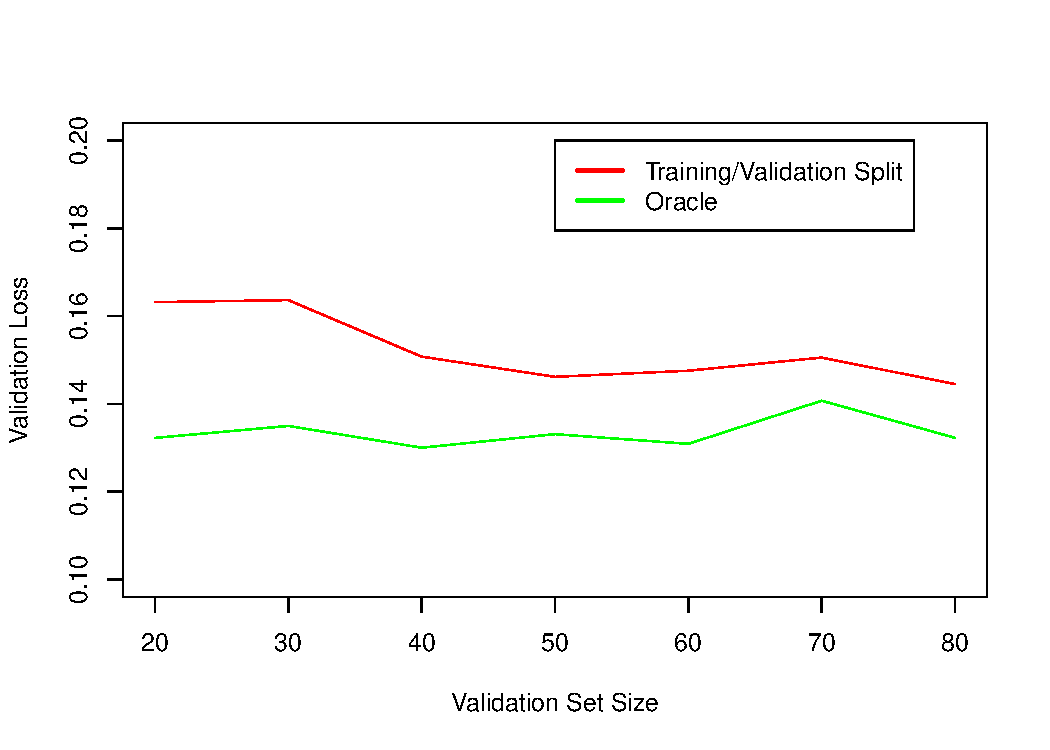
\includegraphics[height=80mm]{../R/figures/validation_size_loss.pdf}
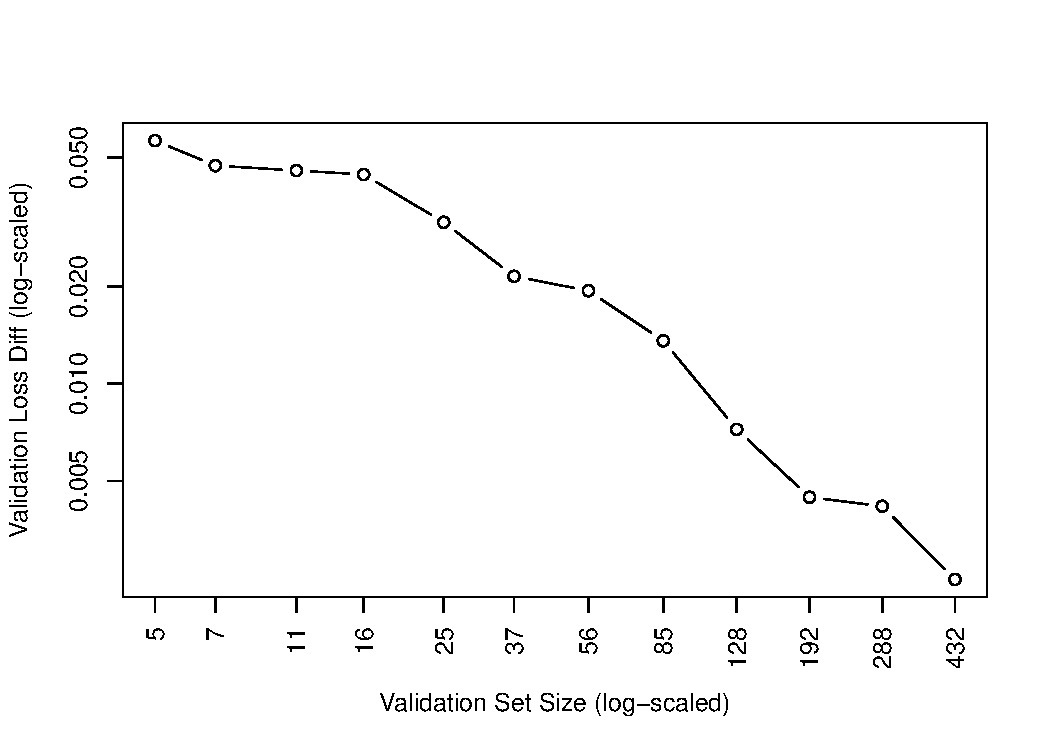
\includegraphics[height=80mm]{../R/figures/validation_size_loss_diff.pdf}
%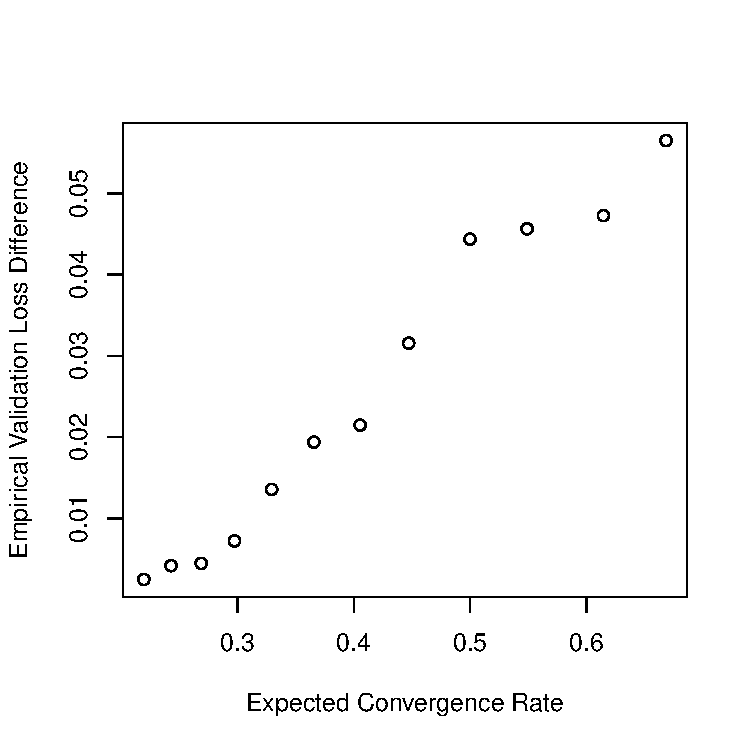
\includegraphics[height=80mm]{../R/figures/qqplot.pdf}
\end{figure}

\section{Discussion}\label{sec:discussion}

In this paper, we have established oracle inequalities for penalty parameter selection using a training/validation split framework or $k$-fold cross-validation. The results address the concern in \citet{bengio2000gradient} regarding ``the amount of overfitting that can be brought when too many hyperparameters are optimized.'' Our results show that 
this should not be a major concern. In a non-parametric setting or parametric setting where $p$ grows with $n$, the oracle error is the dominating term in the upper bound. At worst, the tuning penalty parameter problem contributes an error that is on the same order as the oracle error, say in a parametric setting where $p$ is fixed. 

There is recent interest in combining regularization methods, but seems to be an artificial restriction to two or three penalty parameters. The area of penalized regression methods with tens or hundreds of penalty parameters remains largely unexplored. Our results suggest that this direction of research could be fruitful. As shown in Feng and Simon (TBD), un-pooling the penalty parameters in a sparse group lasso model is surprisingly effective.

One major caveat to our results is that we have assumed that the penalty parameters can be tuned such that the validation loss is minimized. However it is difficult to find the global minimizer since the validation loss is not convex in the penalty parameters. Optimization methods need to be developed to effectively solve the bilevel optimization problems in \eqref{eq:bilevel}. In addition, it would be worthwhile to understand the performance of models that are only local minimizers of the validation loss.

Finally, there are still many open questions to explore. Our results assume that the fitted models are smoothly parameterized with respect to the penalty parameters and we provide a number of examples that satisfy these conditions. There are probably many more examples of regression problems that satisfy the smoothness condition and the smoothness condition itself can probably be generalized.

In addition, it would be interesting to bound the distance between the selected and oracle penalty parameters
\begin{equation}
\label{penalty_diff}
\left \| \hat{\boldsymbol \lambda} - \tilde{\boldsymbol \lambda} \right \|_2
\end{equation}
Such a result would perhaps give a more intuitive understanding of penalty parameter selection methods.


%We find that the difference between the oracle error and the selected model error does not increase dramatically with the number of penalty parameters. the increase in error from tuning parameters model decreases at a near-parametric rate if the fitted models are smoothly parameterized in terms of the penalty parameters. For many penalized regression problems, we find that this is indeed the case. Our results show that adding penalty parameters does not drastically increase the model complexity. This supports recent efforts to combine regularization methods and ``un-pool" regularization parameters. Furthermore, since our result holds for a search over a dense set of penalty parameters, our prediction error bounds apply to cross-validation over a continuum of values, as done in hyper-parameter optimization methods.

\section{The Proof} \label{sec:proofs}

In this paper, we will measure the the complexity of $\mathcal{G}(T)$ by its metric entropy. Let us recall its definition here:

\begin{definition}
Let the covering number $N(u, \mathcal{G}, \| \cdot \|)$ be the smallest set of $u$-covers of $\mathcal{G}$ with respect to the norm $\| \cdot \|$. The metric entropy of $\mathcal{G}$ is defined as the log of the covering number:
\begin{equation}
H (u, \mathcal{G}, \| \cdot \| ) = \log N(u, \mathcal{G}, \| \cdot \|)
\end{equation}
\end{definition}

\begin{theorem}
\label{train_val_thrm_complicated}
Let $\epsilon$ be independent sub-Gaussian random variables.
Suppose that $\sup_{g \in \mathcal{G}} \| g \|_\infty \le G < \infty$.
Suppose for any training dataset $T \subseteq D$ with $\| \epsilon \|_T \le 2 \sigma$, we have
\begin{equation}
\int_0^R H^{1/2} \left ( u, \mathcal{G(\cdot | T)} \| \cdot \|_V \right ) du \le \psi(n, J, \sigma)
\end{equation}

Then for all $\delta  > 0$ such that
\begin{equation}
\sqrt{n_{V}}\delta^{2}
\ge
c \left[
\psi_{T}\left(2\left\Vert \hat{g}_{\tilde{\lambda}}-g^{*}\right\Vert _{V} + 2\delta\right)
\vee
\left(2\left\Vert \hat{g}_{\tilde{\lambda}}-g^{*}\right\Vert _{V}+2\delta\right)
\right]
\end{equation}

Then with high probability, we have
\begin{equation}
\left \|\hat{g}_{\hat{\lambda} }(\cdot | T) - g^* \right \|_V
\le
\min_{\lambda \in \Lambda}\| \hat{g}_{\lambda}(\cdot | T) - g^*\|_V
+ \delta
\end{equation}
\end{theorem}

\begin{proof}
Chaining and peeling.
\end{proof}

%In the penalized regression setting, each function $\hat{g}(\cdot |\boldsymbol \lambda)$ in $\mathcal{G}(T)$ directly maps to a set of penalty parameters, so one would expect that the covering number of $\mathcal{G}(T)$ and $\Lambda$ to be related. In Section \ref{sec:examples}, we show that $\hat{g}(\cdot | \boldsymbol \lambda)$ is smoothly parameterized by $\boldsymbol \lambda$ in many penalized regression problems. Using this result, we apply Theorem \ref{train_val_thrm_complicated} to the specific case of penalized regression to get Theorem \ref{thrm:train_val}.
%
%Note that the complexity term in the upper bound contains a $\log n_V$ term. This is the result of allowing the range of $\Lambda$ to increase at a polynomial rate in the validation set size $n_V$. (Perhaps we should be more explicit and just have $\lambda_{\min} $ and $\lambda_{\max}$)

\paragraph{Proof of Theorem \ref{thrm:train_val}}

\begin{proof}
%By Lemma param\_covering\_cube, we have
%\[
%H(u,\mathcal{G}(T),\|\cdot\|_{V})\le\log\frac{1}{C_{J}}+J\log\left(\frac{2n^{t_{max}-\kappa}+2Cu}{Cu}\right)
%\]
%
%
%Let $R_{1}=R\wedge\sqrt{n^{t_{max}-\kappa}/C}$.
%
%Then after immense algebraic massaging, we get
%\begin{equation}
%\int_{0}^{R}H{}^{1/2}(u,\mathcal{G}(T),\|\cdot\|_{V})du
%\le
%R\left(\left[\log\frac{1}{C_{J}}+J(2+\log4)+J\log\left(\frac{4n^{t_{max}-\kappa}}{C}\right)\right]^{1/2}+\sqrt{2J\log\frac{1}{R}\vee0}\right)
%\end{equation}
%
%We note since $\delta > \frac{1}{n_{V}}$ (modulo a constant), it suffices to choose $\delta$ such that
%\[
%\sqrt{n_{V}}\delta^{2}\ge c\left(\left\Vert \hat{g}_{\tilde{\lambda}}-g^{*}\right\Vert _{V}+\delta\right)\left(\left[\log\frac{1}{C_{J}}+J(1+\log4)+J\log\left(\frac{4n^{t_{max}-\kappa}}{C}\right)\right]^{1/2}+\sqrt{J\log n_{V}}\right)
%\]
%
%Let
%\[
%K=c\left(\left[\log\frac{1}{C_{J}}+J(1+\log4)+J\log\left(\frac{4n^{t_{max}-\kappa}}{C}\right)\right]^{1/2}+\sqrt{J\log n_{V}}\right)
%\]
%and
%\[
%\omega=\left\Vert \hat{g}_{\tilde{\lambda}}-g^{*}\right\Vert _{V}
%\]
%
%The quadratic formula gives us that
%\[
%\delta\ge\frac{K+\sqrt{K^{2}+4K\omega\sqrt{n_{V}}}}{2\sqrt{n_{V}}}
%\]
\end{proof}



\paragraph{Proof of Theorem \ref{thrm:kfold}}

\begin{lemma}
\label{oracle_maintained}
The oracle rate isn't changed when we add the ridge penalty
\end{lemma}

\paragraph{Proof of Lemma \ref{lemma:nonparam_smooth}}
\paragraph{Proof of Lemma \ref{lemma:nonsmooth}}

\paragraph{Proof of Lemma \ref{lemma:parametric}}

\begin{lemma}
\label{lemma:sobolev_prop}
Sobolev penalty has nice properties
\end{lemma}

\paragraph{Proof of Lemma \ref{lemma:sobolev}}

\paragraph{Ridge Perturbations don't change the solution very much - nonsmooth}
\begin{lemma}
	\label{lemma:ridge_perturb_nonsmooth}
	Fitted models are continuous in $w$.
\end{lemma}

\bigskip

\bibliographystyle{agsm}
\bibliography{multi-penalties-theory}

\end{document}
